\chapter{Desenvolvimento das arquiteturas propostas}
\label{cap5}

A documentação do desenvolvimento das arquiteturas propostas é um assunto pertinente para reprodução e\/ou validação dos dados obtidos durante a execução dos testes, além do detalhamento de seu funcionamento.
%
Durante o desenvolvimento foram utilizados padrões de projetos e tecnologias que facilitaram o desenvolvimento de ambas arquiteturas.
%
Neste sentido, o atual capítulo descreve o processo de desenvolvimento das aplicações, a fim de validar as arquiteturas desenvolvidas com base no levantamento teórico realizado neste trabalho.

Inicialmente existe uma preocupação de design de código para garantir que todos os microsserviços contenham a mesma regra de negócio.
%
Este problema é abordado na Sessão~\ref{sec:domain}.
%
Desta forma temos a garantia de que a variação da complexidade dos recursos consumidos ou tempo de latência são de fato da arquitetura empregada no serviço.

Por sua vez, após garantir que não existe variação de complexidade nos algoritmos utilizados nos microsserviços, é descrito as tecnologias utilizadas para a implementação dos microsserviços utilizados pelas arquiteturas. Este tema é abordado na Sessão~\ref{sec:tecnologias_utilizadas}.

\section{Domínio dos microsserviços}
\label{sec:domain}

Para a execução dos testes, existe a necessidade de garantir que todas as aplicações tenham a mesma regra de negócio.
%
Esta necessidade é explícita para garantir que a única variação entre as arquiteturas é o modelo de comunicação entre os microsserviços, não tendo variação pela complexidade da sua regra de negócio.
%
Dessa forma é possível garantir dados justos e homogênios entre ambas arquiteturas.

Para resolver esta demanda, foi utilizado o \textit{Clean Architecture}~\cite{Martin2017Sep}. Tal padrão de projeto visa modularizar em camadas, tal qual o código torne-se reaproveitável e de fácil a substituição.
%
Esta arquitetura pode-se ser visualizada na Figura~\ref{fig:clean_arch}.

\begin{figure}[htb!]
\caption{Modelo teórico de uma aplicação utilizando Clean Architecture.}
\label{fig:clean_arch}
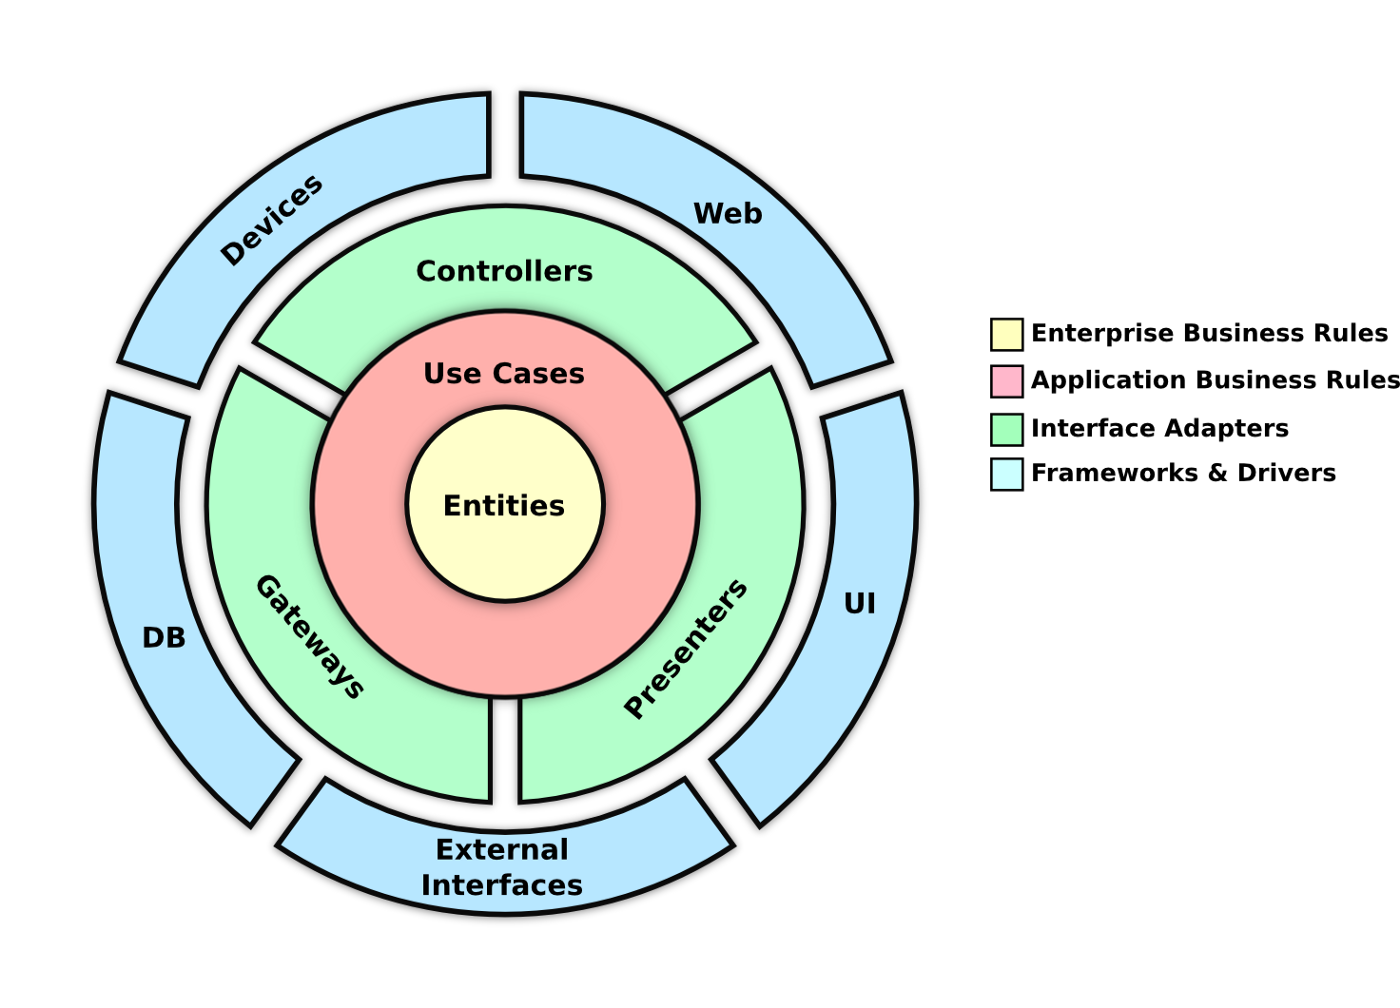
\includegraphics[width=\textwidth]{figuras/clean_architecture.png}
\centering

Autor:~\cite{Martin2017Sep}.
\end{figure}

Este modelo de programação, visível na Figura~\ref{fig:clean_arch} mantém o código fonte da aplicação separado em camadas bem isoladas por interfaces.
%
Esta arquitetura foi construída para utilizar o paradigma de programação orientado a objetos, porém não é restrito a tal paradigma~\cite{Martin2017Sep}.
%
O pacote de domínio real utilizado pode ser visualizado na Figura~\ref{fig:domain_deps}.

\begin{figure}[htb!]
\caption{Árvore de dependências do domínio.}
\label{fig:domain_deps}
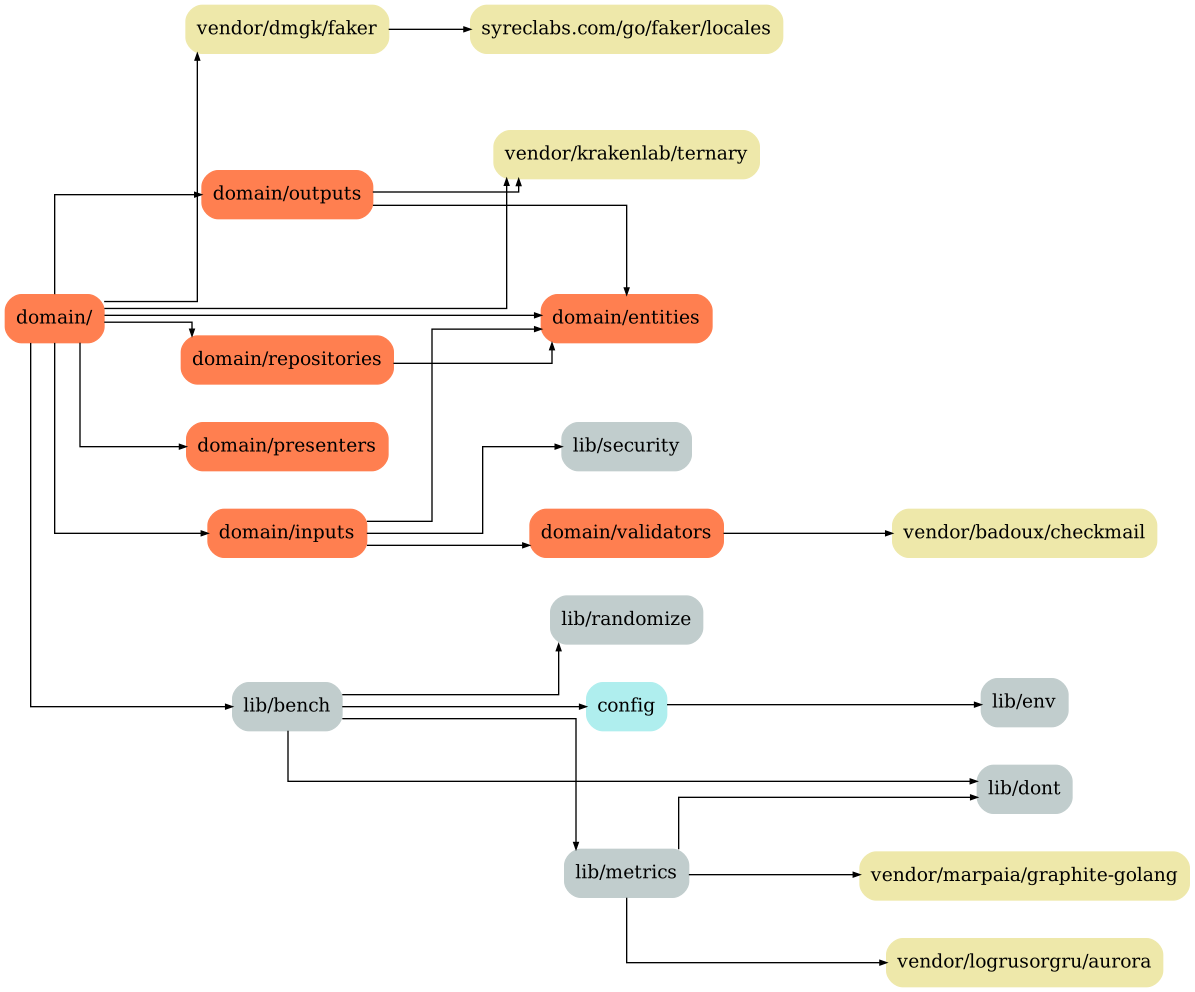
\includegraphics[width=\textwidth]{figuras/deps/domain.png}
\centering

Fonte: O próprio autor.
\end{figure}

Como visível na Figura~\ref{fig:domain_deps}, o domínio gerencia modelos, regras e microsserviços comuns a qualquer aplicação.
%
No domínio das aplicações possuem 3 principais pacotes utilizados para a modularização de fonte de dados e troca de comunicação de microsserviços.
%
São eles:

\begin{itemize}
  \item Repositórios: Este módulo permite trocar a fonte de dados. Pode-se escrever classes que realizam a chamada a outros serviço (padrão de projeto \textit{Proxy}) ou a conexão direta a fonte de dados real.
  \item Entrada: Este módulo possui as estruturas de dados a são convertidas de \ac{json} em microsserviços \textit{web} ou de binário em microsserviços \ac{rpc}. Após a conversão, realizada pela camada externa da infraestrutura, tal dado é utilizado como entrada neste serviço.
  \item Saída: Este módulo possui as estruturas de dados que são serializadas para \ac{json} em microsserviços \textit{web} ou binário em microsserviços \ac{rpc}. Este é o meio de comunicação no código de \textit{Cliente para Serviço} ou \textit{Serviço para Serviço}.
\end{itemize}

A partir destes pacotes, são implementados microsserviços \textit{web} e \ac{rpc} que configuram o domínio e inicializam as istâncias que necessitam para operar tal qual a definição teórica.
%
Dessa forma, após observar o modelo do núcleo de todos os microsserviços implementados, pode-se descrever tecnologias, linguagem de programação e disposição do microsserviços.

\section{Tecnologias Utilizadas}
\label{sec:tecnologias_utilizadas}

Ao redor do domínio da aplicação, diversas tecnologias diferentes são utilizadas para comunicação e armazenamento de dados.
%
Além de tecnologias diretas, foram utilizadas tecnologias para implantação e automatização para auxilio no desenvolvimento dos microsserviços.

Foi eleito a linguagem Golang para programação dos microsserviços.
%
Esta escolha foi realizada por conta da linguagem ser focada em desempenho e velocidade de implementação.

Para armazenamento de dados permanente é utilizado o banco de dados PostgreSQL.
%
Trata-se de um banco de dados \ac{acid}, com modelo de tabelas a qual utiliza a linguagem \ac{sql} para consulta dos dados.
%
